\documentclass[]{finalproject}
\usepackage[algoruled, linesnumbered, noline]{algorithm2e}
\usepackage{float}
\usepackage{graphicx}
\usepackage{minted}
\usepackage{ragged2e}
\graphicspath{{./img}}

\usepackage[parfill]{parskip}
\let\circledS\undefined % here - PS
\usepackage{amssymb}
\usepackage{enumitem}
\usepackage{caption}

\captionsetup{labelfont={bf}}

% Title (and subtitle) of the project
\title{Quicksort}
\subtitle{}

% Group members for the final project (comment out the unnecessary entries)
\begin{groupmembers}
\studentA{Pratyai}{}{Mazumder}
\studentB{Lodovico}{}{Mazzei}
\studentC{Michele}{}{Chersich}
\end{groupmembers}

\abstract {
A short abstract summarising what your project is about and the main results you obtained.
}


\begin{document}
\maketitle

\section{Introduction} \label{introduction}

Sorting is a ubiquitous problem in computer science, with applications in practically every subfield -- data structures, computation geometry, search engines, just to give a few examples.

The sorting problem can be defined as the reordering of a sequence of elements, based on some ordering criterion. More specifically, to be able to sort it, a sequence must possess following two properties\footnote{Either of these requirements can be relaxed for a relaxed variant of the sorting problem. Additionally, for quicksort, we require the list to be \textit{randomly accessible}.}:

\begin{itemize}
\item Its elements are \textit{swappable}: So that the list can be permuted in-place\footnote{I.e. modifying the original sequence object, instead of creating a new one.}.
\item Any two of its elements are \textit{comparable}: I.e. the elements have total ordering.
\end{itemize}

While it can be shown that the lower bound of any comparison sorts is $\Omega(n\log n)$ \cite[p.~193]{clrs} with respect to the input size, there have been many different algorithms invented with different approaches to the comparison sorting problem. Quicksort, originally invented in 1962 by C. A. R. Hoare, is still one of the most commonly used sorting algorithms. There are many variants of the quicksort algorithm, however, we will only focus on one representative example.

\section{The algorithm}


\subsection{The partitioning problem}

Quicksort belongs to the family of \textit{partition sort} algorithms,
where a partitioning routine is called recursively until a whole sequence is sorted.

Given an array $A[1,.....,N]$, the partitioning algorithm should split a permutation
of it, $A'$, into two partitions $U=A'[1,.....,p]$ and $V=A'[p+1,.....,N]$ such that
$U[i] \leq V[j] \;\, \forall \; i,j \in \{[1,p] , [p+1,N]\}$.
By recursively partitioning U and V themselves, base cases will eventually be reached,
consisting of single-element or empty arrays, which are already sorted.
Figure \ref{fig:rec-part} illustrates the recursive routine.

\begin{figure}[H]
    \centering
    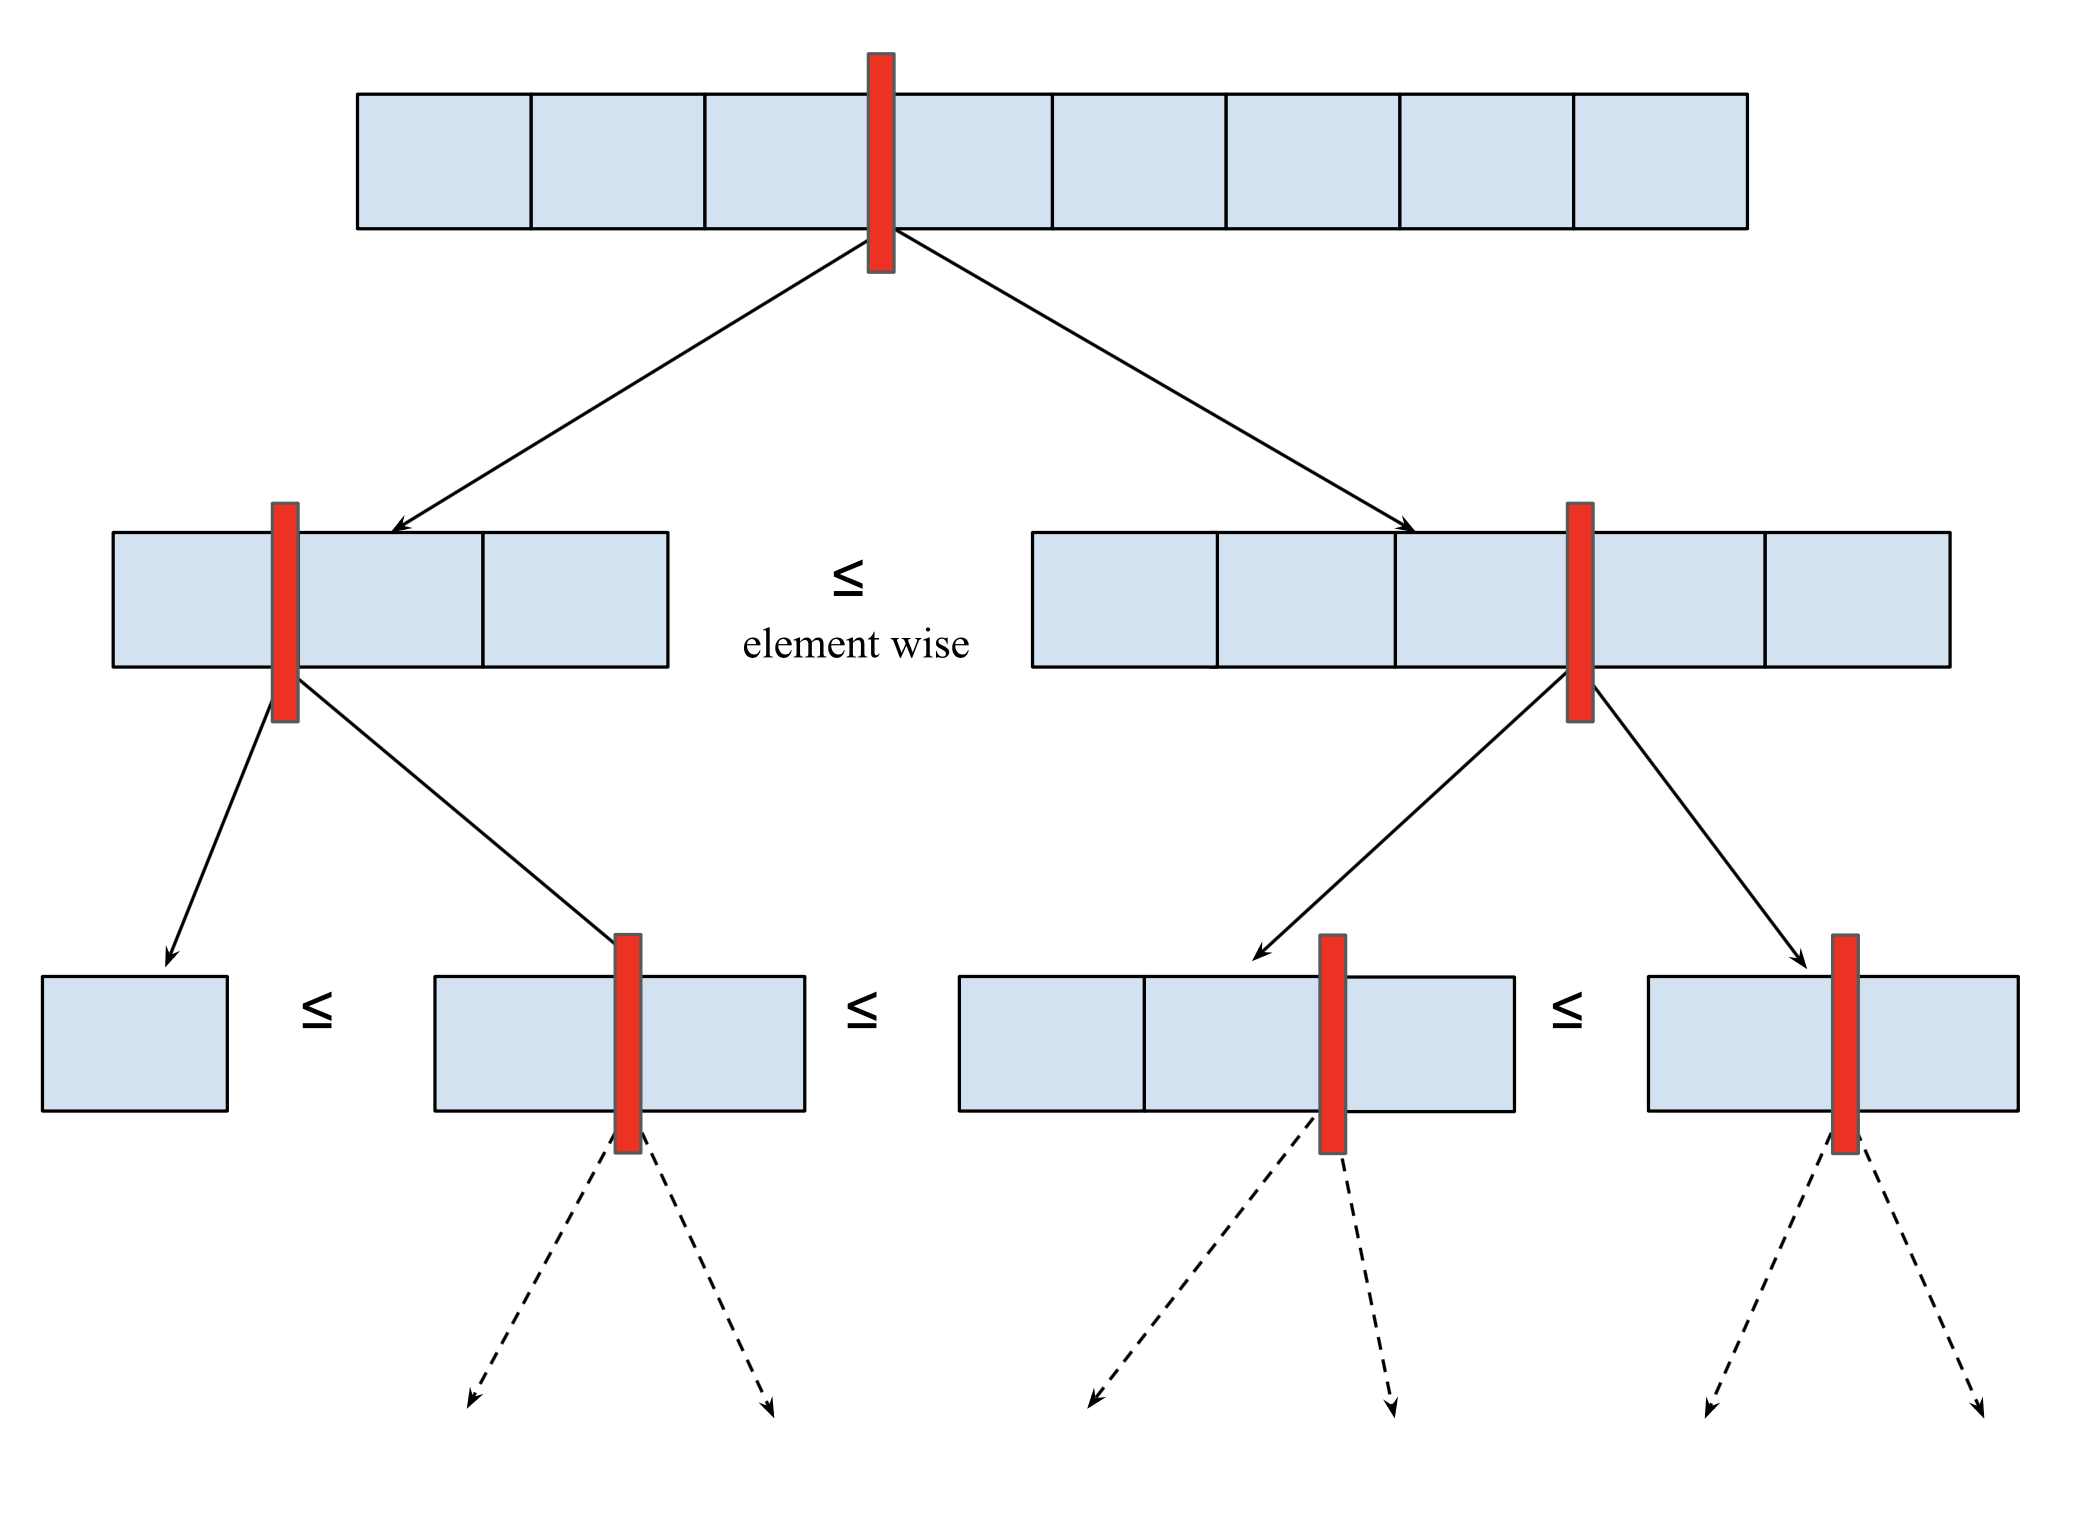
\includegraphics[width=0.6\textwidth]{recursive_partitioning.png}
    \caption{Tree representation of a partitioning process.
    At each level the array(s) are permuted and split into two subarrays, where the condition holds that individual elements in one of them are larger or equal than those in the other.
    The base case of a branch is reached when an array is reduced to one or zero elements.}
    \label{fig:rec-part}
\end{figure}

The following pseudocode recursively sorts a given subarray of $A$. It assumes a partition routine which will be discussed in the following sections.

\begin{algorithm}
	\caption{Quicksort ($A$, $low$, $high$)}
	\label{alg:p1}
	\If(){$low \geq 0 ~\&\&~ high \geq 0 ~\&\&~ low < high$}{p := partition(A, low, high)\\
	quicksort(A, low, p-1)\\
	quicksort(A, p+1, high)}
\end{algorithm}


\subsection{Pivot selection}
The partitioning in quicksort relies on a method called pivoting. This consists in picking a value $\gamma$ to be our pivot. Given the array $A$, we then permute it in a way such that every element before $\gamma$ is smaller than it, and every one after it is larger. The internal order in these subarrays is irrelevant, as it will be addressed in further iterations of the algorithm.\\
Clearly, the pivot choice will have an impact on the efficiency of the algorithm. We divide the selection methods into two categories: one-step and multi-step.\\
The following paragraphs provide a description using as an example the array $A[1,.....,N]$ introduced above.

\subsubsection{One-step selection}
These methods only require chosing a value at each iteration and using it as the pivot, the difference being the position of $A$ from which the value is selected.\\

\begin{itemize}[partopsep=0pt, parsep=0.3pt, topsep=-\parskip, itemsep=1pt]
\item{\textit{First element}}: set the pivot to be the value $A[1]$.\\
\item{\textit{Last element}}: set the pivot to be the value $A[N]$.\\
\item{\textit{Central element}}: set the pivot to be the value $A[\lfloor \frac{(N+1)}{2} \rfloor]$ or $A[\lceil \frac{(N+1)}{2} \rceil]$ if N is even, and $A[\frac{N+1}{2}]$ if N is odd.\\
\item{\textit{Random element}}: set the pivot to be value $A[r]$, where $r$ is a random number such that $1 \leq r \leq N$.
\end{itemize}

\subsubsection{Multi-step selection}
Given that the most efficient case of the partitioning is achieved when picking the median, the following methods involve computing the median of some odd sample of values extracted from the array. The difference among the methods lies in the positions of the array from which the values are taken, and in the sample size. The latter is indicated by the suffix $T$, with most common implementations using $3 \leq T \leq 9$.\\

\begin{itemize}[partopsep=0pt, parsep=0pt, topsep=-\parskip, itemsep=0pt]
\item{\textit{Median-of-T with fixed selection:}} $T$ integers $1 \leq n_{1},....,n_{T} \leq N$ are fixed beforehand. The median of $\{A[n_{1}],.....,A[n_{T}]\}$ is then computed and used as the pivot for the partitioning.\\
\item{\textit{Median-of-T with random selection:}} $T$ random integers $1 \leq r_{1},....,r_{T} \leq N$ are generated. The median of $\{A[r_{1}],.....,A[r_{T}]\}$ is then computed and used as the pivot for the partitioning.
\end{itemize}

\subsection{Partitioning around the pivot}
There are a variety of procedures to partition a list around a pivot, however, the most commonly used in quicksort are the Lomuto scheme and the Hoare scheme.
We will be describing and showing the latter, though it is straightforward to see how some modifications would still achieve the same result.\\
Figure 2 illustrates the process of partitioning around a chosen value, the number 4 in this case. Recalling from the previous paragraph, this could have been a one-step selection using a random index.\\
Once the pivot value is selected, we set two iterators $i$ and $j$, which are initialized respectively at values $0$ and $N+1$.\\
Iterator $i$ will always check if the value $A[i] < 4$, whereas $j$ will check if $A[j] \geq 4$.\\
The algorithm then proceeds as follows:\\

\begin{itemize}[partopsep=0pt, parsep=0.3pt, topsep=-\parskip, itemsep=1pt]
  \item{} \textit{i} increases in steps of 1 until $A[i]$ is not compliant with its condition. It will then stop.
  \item{} \textit{j} decreases in steps of 1 until $A[j]$ is not compliant with its condition. It will then stop.
  \item{} the condition $j>i$ is checked. If not met, the partitioning is complete and the algorithm halts, otherwise it proceeds.
  \item{} the values $A[i]$ and $A[j]$ are swapped.
  \item{} repeat from step one.
\end{itemize}


\begin{figure}[H]
  \begin{center}
   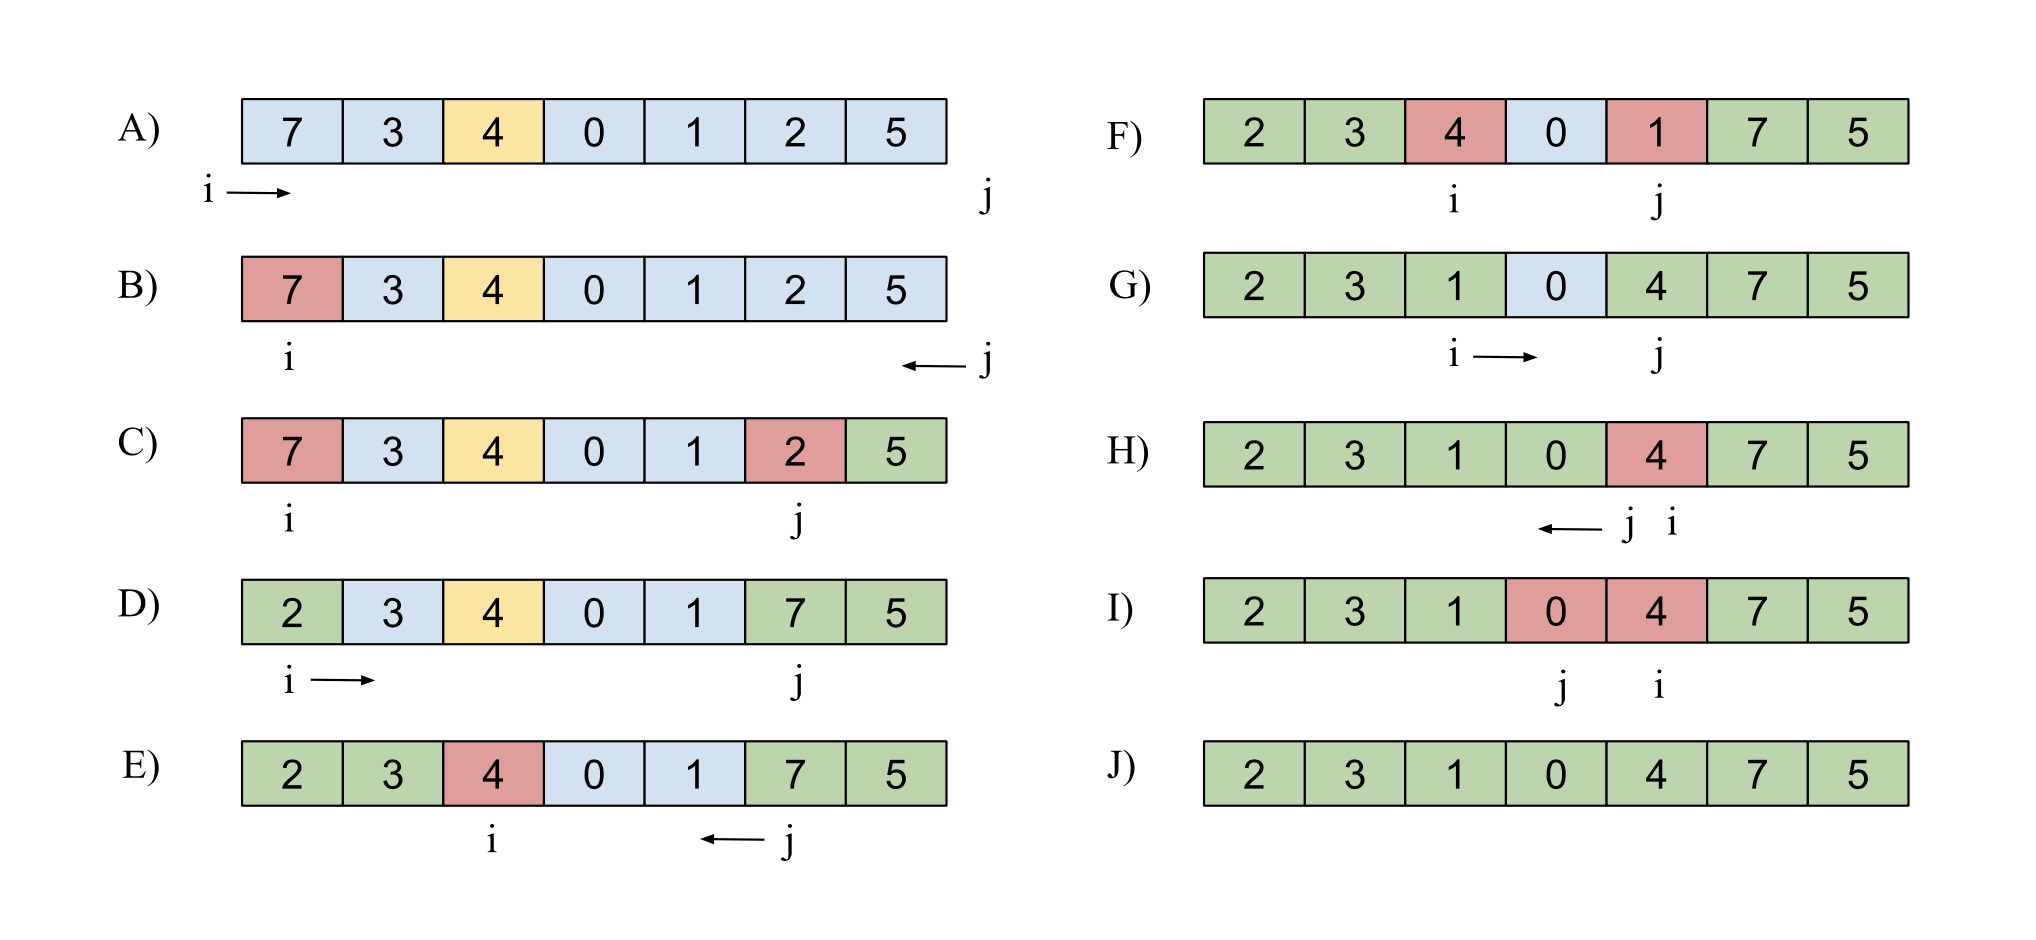
\includegraphics[scale=0.5]{img/pivot_partitioning.png}
  \end{center}
  \caption{Partitioning of the array around the chosen pivot $p=4$, in yellow.
  Blue elements have not been checked yet; red elements are not compliant and yet to be swapped; green elements are in a compliant position and require no more actions. \\
  \textbf{A)} \textit{i} begins by increasing and stops at the first step, as $7 \ngeq 4$.
  \textbf{B)-C)-D)} \textit{j} starts decreasing until it encounters $2 \ngeq 4$. Condition $i<j$ is verified, so values $A[i]=7$ and $A[j]=2$ are swapped.
  \textbf{E)} \textit{i} increases up to the value $4 \nless 4$.
  \textbf{F)-G)} \textit{j} decreases until it finds $1 \ngeq 4$. Condition $i<j$ is verified, so values $A[i]=4$ and $A[j]=1$ are swapped.
  \textbf{H)} \textit{i} increases and stops at $4 \nless 4$.
  \textbf{I)-J)} \textit{j} increases and stops at $0 \ngeq 4$. Condition $i<j$ is not verified, so the algorithm ends. \\
  Note that all elements to the right of the pivot 4 are greater or equal than it, and all the ones to its left are smaller than it.
  By recursively repeating this process on the subarrays on each side of the pivot (excluding the pivot itself), an entirely sorted array will be obtained in the end.}
\label{fig:rec-part2}
\end{figure}

The alorithm from Figure \ref{fig:rec-part2} is recapitulated in the following pseudocode.

\begin{algorithm}
	\caption{partition($A$, $low$, $high$)}
	\label{alg:p2}

	pivot = selectPivot(A)

	i, j := low - 1, high + 1

	loop forever

	\Indp

	do i := i + 1 while $A[i] < pivot$

	do j := j - 1 while $A[j] \geq pivot$

	\If(){$i \geq j$}{return}

	swap A[i] with A[j]
\end{algorithm}



\section{Complexity analysis}

We will consider the notion of algorithm complexity\footnote{Reference?} to be the growth of its computational cost with respect to some input parameters. In general the cost can be any runtime resources the algorithm needs. Here, we will restrict the analysis to an estimation of how fast the computation time will grow as the size of the input sequence increases.

We will also assume an extremely simplified model of execution\footnote{Reference?} that ignores considerations like cache, locality of reference, hardware architecture -- all of which have significant impact on computation time. In this model, the only relevant sources of computational cost are the two operations -- comparison and swap -- each costing a single unit of time; everything else, including the recursive function calls and random number generations, are considered relatively insignificant.

\subsection{Analysis of \texttt{partition} routine}

Let's consider the Hoare partitioning scheme outlined in \textbf{Pseudocode \#2}. The first operation is selecting a pivot element from the sequence which is $\Theta(1)$ for every pivot selection method described in \textbf{Section \#1}.

Once the pivot is selected, we  are scanning the subarray under consideration\footnote{Or the whole array if this is the outermost call in the recursion.}, starting with a pointer in each boundary and moving one of the pointers towards the other in each step. Each step has exactly one comparison between the current pointees, one occasional comparison between the pointers themselves to check if they have met already, and one occasional swap between the current pointees -- i.e. each step is $\Theta(1)$.

Since we can move the pointers $n$ times, we have exactly $n$ steps in a single call to the \texttt{partition(A, low, high)}, where $n = high - low + 1$ is the length of the subarray. Therefore, the total complexity of the \texttt{partition} routine is: $$T_{partition}(n) = \Theta(1) + n\Theta(1) = \Theta(n)$$

This complexity estimation holds true for all the pivot selection schemes and the partitioning schemes we have discussed, and also for any input data.

\subsection{Analysis of \texttt{quicksort} routine}

Now, let's consider the recursive \texttt{quicksort} routine outlined in \textbf{Pseudocode \#1}. The first operation is a $\Theta(1)$ comparison to check if it is a base case. A base case requires no additional computation, i.e. $\Theta(0)$.

Otherwise, we incur exactly one call to the \texttt{partition} routine and two calls to the \texttt{quicksort} routine with the two partitions. I.e. if the two partitions have sizes $u$ and $n-u$, the complexity of the \texttt{quicksort} routine is: $$T(n) = T_{partition}(n) + T(u) + T(n-u-1) = T(u) + T(n-u-1) + \Theta(n)$$

This is a recursive formula where the partition sizes, $u$ and $n-u-1$, depends on the input data and the pivot selection method. So, to get an explicit formula without the recursion, we need to consider different input and pivot scenarios. We will do this for the following two important cases, which are also the most typical for complexity analysis.

\subsubsection{Worst-case analysis}

The worst case for the \texttt{quicksort} routine is when the partitions are the least balanced, i.e. the pivot element ends up being the largest or the smallest in the subarray under consideration. So,
\begin{align*}
T_{worst}(0) &= \Theta(1) \\
T_{worst}(1) &= \Theta(1) \\
T_{worst}(n) &= T_{worst}(n-1) + T_{worst}(0) + \Theta(n) \\
\intertext{Expanding this recurrence until the base case, we find,}
T_{worst}(n) &= \sum_{k=1}^n\Theta(k) = \Theta(n^2)
\end{align*}

\subsubsection{Average-case analysis}

For deterministic pivot selection methods, there is always some hostile input data for which the algorithm will take the worst case. However, in practical scenarios, running into a hostile input data is fairly unlikely. We are often interested in the average case analysis that accounts for the prior distribution of the input data to compute the average cost.

Since the location of the pivots determines the runtime of quicksort for a given input data, we will consider a prior distribution of the pivot location at each call to \texttt{quicksort} routine. Let it be uniform -- i.e. if the size of the given array is $n$ and we don't have any other information about the pivot, we assume it can be $k^{th}$ smallest element for any $k = 1, ..., n$.
\begin{align*}
T(n) &= \frac{1}{n}\sum_{k=1}^{n}\big(T(k-1) + T(n-k)\big) + \Theta(n) \\
&= \frac{1}{n}\big(\sum_{k=1}^{n}T(k-1) + \sum_{k=1}^{n}T(k-1)\big) + \Theta(n) \\
&= \frac{2}{n}\sum_{k=0}^{n-1}T(k) + cn ~~~~~[\text{for some constant $c$}]\\
\implies nT(n) &= 2\sum_{k=0}^{n-1}T(k) + cn^2 \\
\implies nT(n) - (n-1)T(n-1) &= 2T(n-1) + 2cn - c ~~~~~[\text{Subtracting $(n-1)T(n-1)$ from $nT(n)$}]\\
\implies nT(n) &\approx (n+1)T(n-1) + 2cn \\
\intertext{From this recurrence we get the set of equations,}
\frac{T(n)}{n+1} &= \frac{T(n-1)}{n} + \frac{2c}{n+1} \\
\frac{T(n-1)}{n} &= \frac{T(n-2)}{n-1} + \frac{2c}{n} \\
&\vdots \\
\frac{T(2)}{3} &= \frac{T(1)}{2} + \frac{2c}{3} \\
\intertext{Adding up them yields,}
\frac{T(n)}{n+1} &=  \frac{T(1)}{2} + 2c \sum_{k=3}^{n+1}\frac{1}{k} = \frac{T(1)}{2} + 2c(\log(n+1) + \gamma - \frac{3}{2}) ~~~~~[\text{$\gamma \approx 0.577$ is the Euler's constant}] \\
\implies T(n) &= \mathcal{O}(n\log n)
\end{align*}

\subsection{Analysis of randomized Quicksort}

\section{Parallel processing}
\subsection{Scaling features}
\subsection{Parallelizing Quicksort}

\section{Computational geometry and the convex hull problem}
Computational geometry is the study of algorithms for the solution of geometric problems in the Euclidean space \cite{paper}.
The convex hull problem belongs to this class of problems, and has a wide range of applications across several disciplines
(e.g. data classification, collision avoidance, image processing and recognition). It is defined as follows:
given a set of points, find the smallest convex polygon containing all the points \cite{geowiki}.
For the purpose of this project, we will consider only the planar convex hull, with 2D Cartesian coordinates.

\subsection{The Quickhull algorithm}
The Quickhull algorithm is a variation of Quicksort for the solution of the convex hull problem.
The algorithms works as follows:
an initial partitioning step is done by picking the leftmost and rightmost point.
Let these two points be $p_1$ and $p_2$, respectively.
The line connecting $p_1$ and $p_2$ splits the set in two parts.
For each subset, we search for the farthest point from the line: let this point be $p_{max}$.
If it exists, the points lying inside the triangle $p_1p_2p_{max}$ are removed from the set,
and the recursive step is applied on the points that lie outside the lines $p_1p_{max}$ and $p_2p_{max}$.
Again, let $p_1$ and $p_2$ be the end points of the line in the recursive step.
The stop condition occurs when $p_{max}$ is not found, as there are no points outside $p_1p_2$.
The very first steps of the algorithm are illustrated in Figure \ref{fig:qh-steps}.
The pseudocode is given in Algorithms \ref{alg:qh1} and \ref{alg:qh2}.

\begin{figure}[H]
    \centering
    \begin{minipage}{.33\linewidth}
		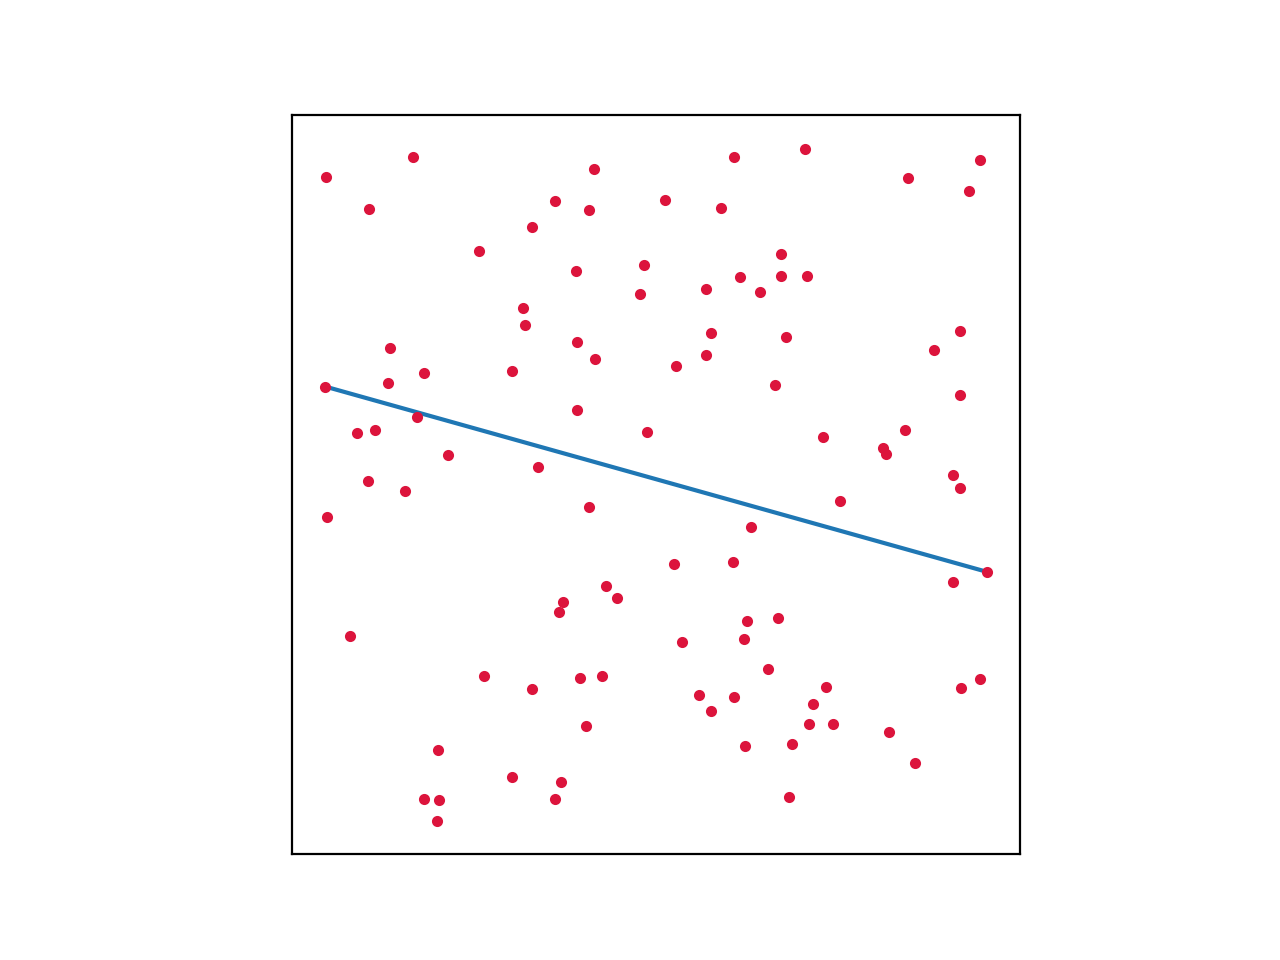
\includegraphics[width=\linewidth]{quickhull1.png}
	\end{minipage}
	\begin{minipage}{.33\linewidth}
		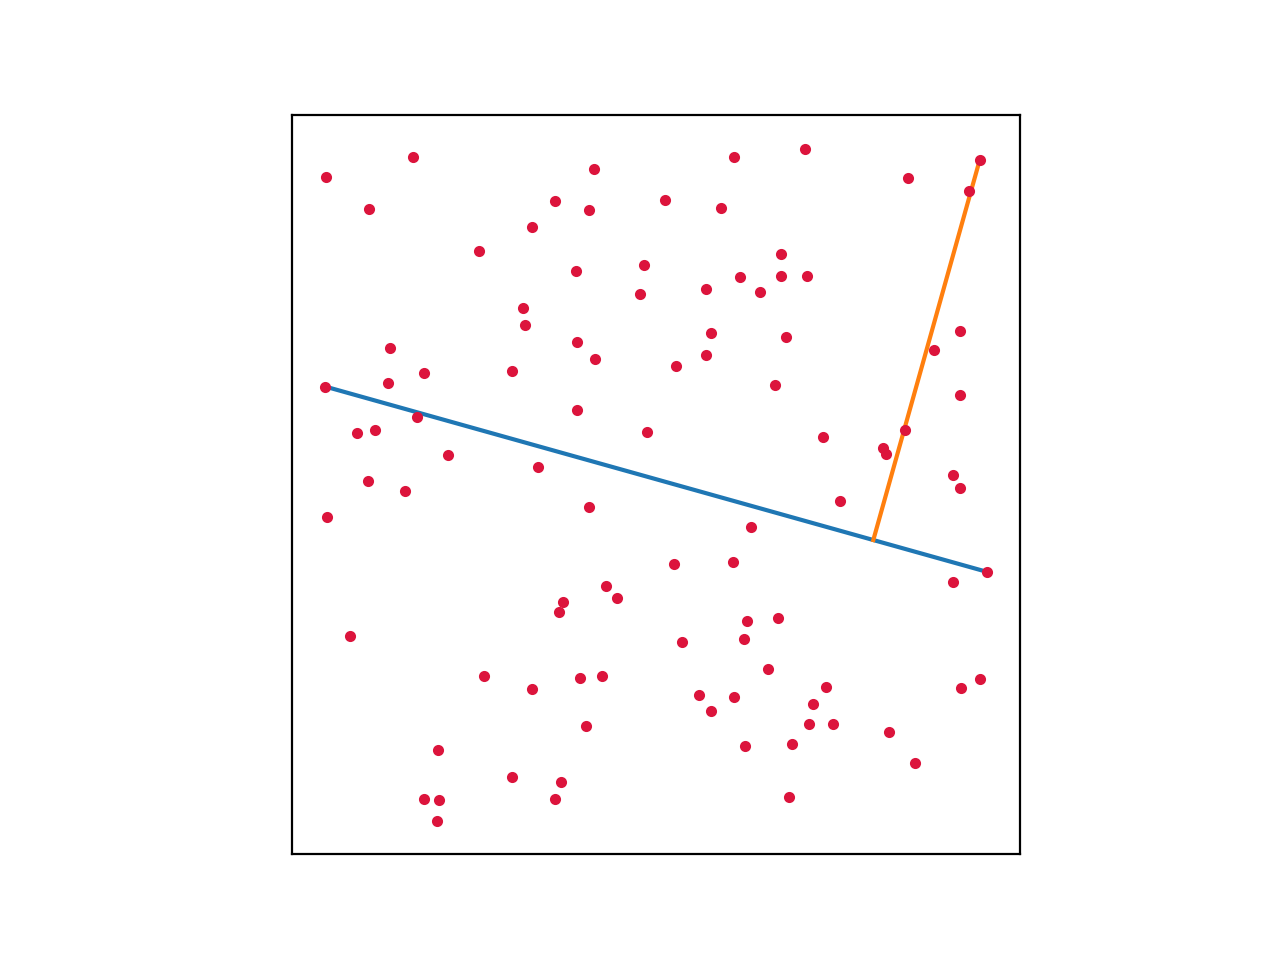
\includegraphics[width=\linewidth]{quickhull2.png}
	\end{minipage}
    \begin{minipage}{.33\linewidth}
		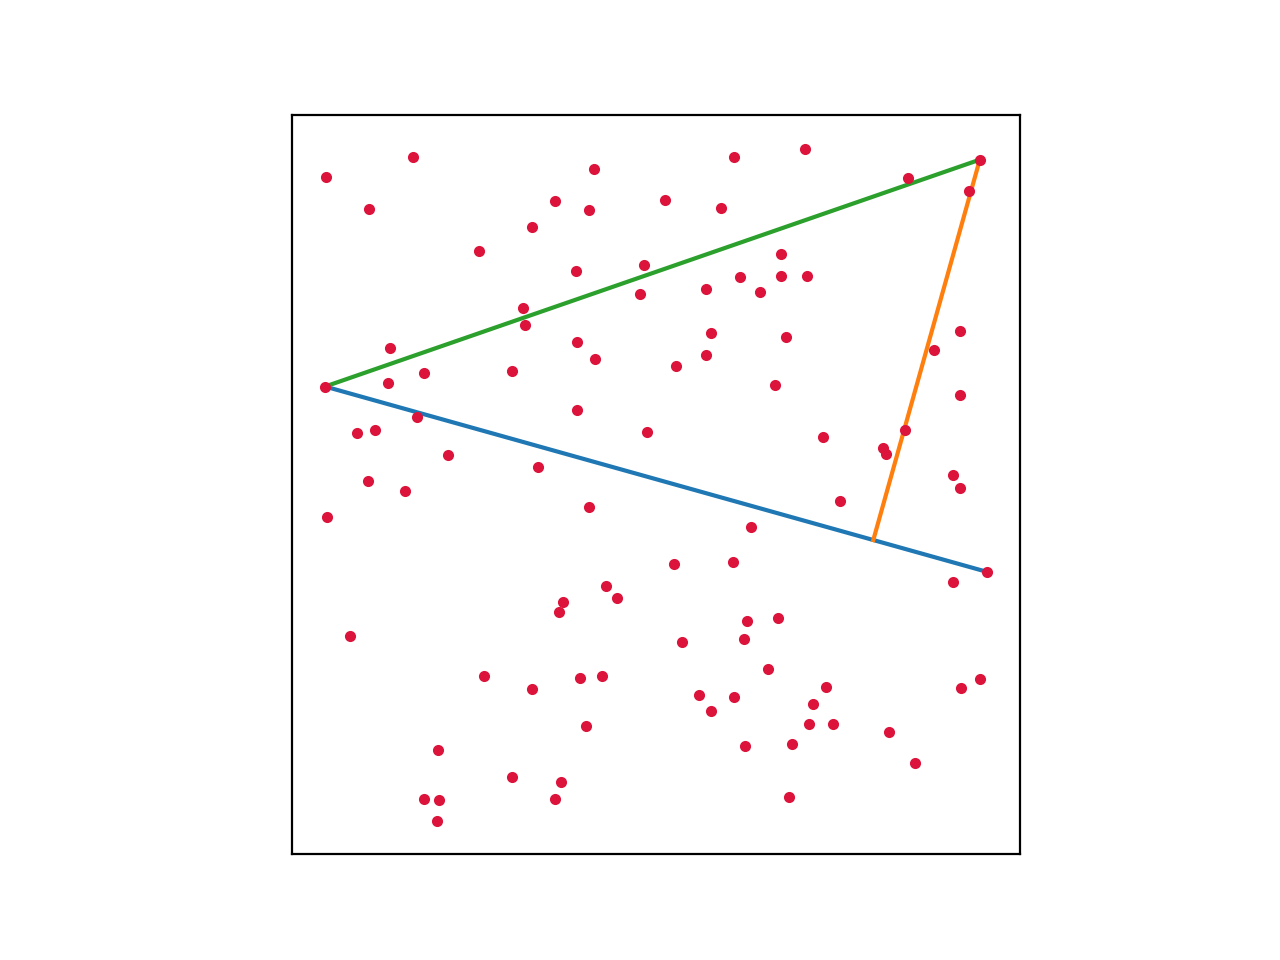
\includegraphics[width=\linewidth]{quickhull3.png}
	\end{minipage}
    \caption{Three steps of the Quickhull algorithm: the line $p_1p_2$ partitions the set of points in two subsets (left); the farthest point $p_{max}$ from the line is found (middle); the triangle $p_1p_2p_{max}$ shrinks the solution set (right).}
    \label{fig:qh-steps}
\end{figure}

\begin{algorithm}
    \caption{Quickhull ($P$)}
    \label{alg:qh1}
    P is a set of points with (x, y) coordinates

    Find the points $p_1$ and $p_2$ with x-coordinates $x_{min}$ and $x_{max}$

    Quickhull\_onside($P$, $p_1$, $p_2$, $1$)

    Quickhull\_onside($P$, $p_1$, $p_2$, $-1$)
\end{algorithm}
\begin{algorithm}
  \caption{Quickhull\_onside ($P$, $p_1$, $p_2$, $s$)}
  \label{alg:qh2}
  Let $p_{max}$ be the the point that is farthest from the line $p_1p_2$, on side $s$.

  \If(){$p_{max}$ does not exist}{return}

  Remove from $P$ all points that lie in the triangle $p_1p_2p_{max}$

  Let $s_1$ and $s_2$ be the outer sides of lines $p_1p_{max}$ and $p_2p_{max}$

  Quickhull\_onside($P$, $p_{max}$, $p_1$, $s_1$)

  Quickhull\_onside($P$, $p_{max}$, $p_2$, $s_2$)
\end{algorithm}

We can observe how Quickhull, just like Quicksort,
is both a divide-and-conquer and a sorting algorithm. The former approach is implemented by partitioning,
splitting the initial problem into smaller subproblems in a recursive fashion, whereas the latter is applied by comparing
Euclidean distances between points. Again, the complexity is $O(n^2)$ in the worst case and $O(n\log{n})$ in the average case.

\subsection{Distributed Quickhull}
The Quickhull algorithm is sequential by design,
as each recursive call depends on the previous ones for the computation of the solution set \cite{qhpaper}.
Therefore, parallelizing the algorithm by multithreading is not feasible, as it is not possible to independently compute the solution to subproblems.
However, the set of points can be distributed over multiple processes, and inter-process communication can be used to combine the partial results.\\
The pseudocode of the distributed version of Quickhull is given in Algorithm \ref{alg:qh3}.

\begin{algorithm}
  \caption{Distributed Quickhull ($P$)}
  \label{alg:qh3}
  Each process computes the points with minimum and maximum x-coordinate among their local portion of the dataset, then the global minimum and maximum are computed, and broadcast to all processes (\textit{allreduce}).

  Each process computes the farthest point from the line joining the two points, and the global result is found (\textit{allreduce}).

  Once each process has all three vertices of the triangle, they can remove the points that lie inside the triangle from their dataset.

  The recursive step is repeated just like in the sequential version.

  At the end, the solution is scattered over all processes, so it must be gathered on the root process (\textit{gather}).
\end{algorithm}

As we can see, the procedure is almost identical to the sequential version.
The key difference is the use of interprocess communication in the partitioning steps:
the computation performed by each process to find the leftmost and rightmost points, as well as the farthest point at every iteration,
is limited to a subset of points, so the results of all processes must be combined, in order to obtain the global result.
Note that communication is used just for the aforementioned purpose, and to combine the final solution on the root process,
keeping the communication cost low.

\subsubsection{Scaling analysis}
Running the algorithm for large input sizes with different numbers of processes, we can observe significant gains in performance.
A scaling chart is reported in Figure \ref{fig:qh-scaling}.
\begin{figure}[H]
    \centering
    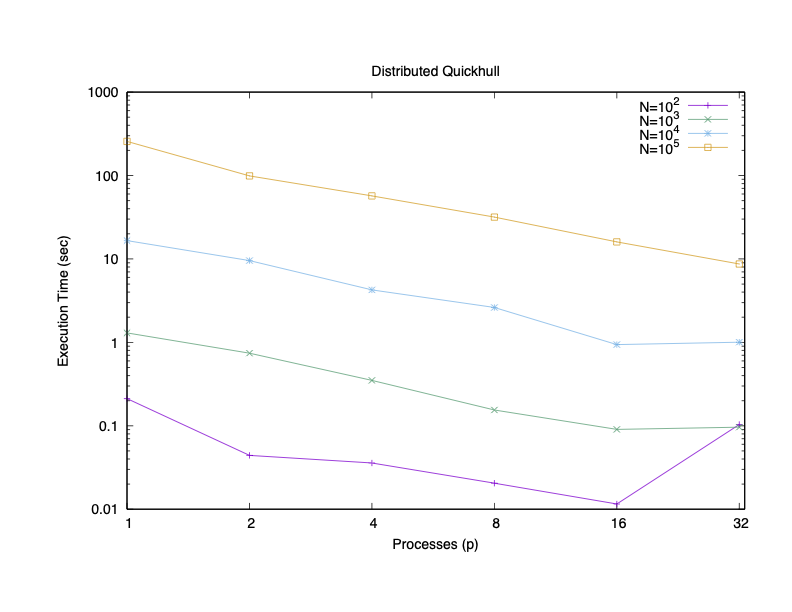
\includegraphics[width=0.6\linewidth]{gpStrongTime.png}
    \caption{Performance scaling of distributed Quickhull.}
    \label{fig:qh-scaling}
\end{figure}

We can observe the gain in performance obtained by the distributed version of the algorithm:
by doubling the number of processes, the execution time roughly halves.
However, we can also observe the effect of over-parallelizing with respect to the problem size:
e.g. for $N=10^2$, 32 processes perform worse than 16.

%%%%%
\clearpage
\bibliographystyle{abbrv}
\bibliography{references}



\end{document}
